%% Template for ENG 401 reports
%% by Robin Turner
%% Adapted from the IEEE peer review template

%
% note that the "draftcls" or "draftclsnofoot", not "draft", option
% should be used if it is desired that the figures are to be displayed in
% draft mode.

%\documentclass[12pt]{IEEEtran}
\documentclass[12pt, letterpaper]{article}
\usepackage{cite} % Tidies up citation numbers.
\usepackage{url} % Provides better formatting of URLs.
\usepackage[utf8]{inputenc} % Allows Turkish characters.
\usepackage{booktabs} % Allows the use of \toprule, \midrule and \bottomrule in tables for horizontal lines
\usepackage{graphicx}

\usepackage{amsmath}
\usepackage{amssymb}
\usepackage{mathtools} 
\usepackage{listings}
\usepackage{enumitem}
\usepackage{tikz}
\usetikzlibrary{shapes.geometric, arrows}
\usetikzlibrary{positioning,fit,calc}
\usepackage{calc}

\usepackage[colorlinks]{hyperref}
\hypersetup{
    colorlinks=true,
    linkcolor=blue,
    filecolor=magenta,      
    urlcolor=cyan,
    pdftitle={Overleaf Example},
    pdfpagemode=FullScreen,
    }


\hyphenation{op-tical net-works semi-conduc-tor} % Corrects some bad hyphenation 

\newcommand{\mtrx}[1]{\begin{bmatrix}#1\end{bmatrix}}

\graphicspath{ {./images/}  }


\begin{document}

% Define block styles
\tikzstyle{decision} = [diamond, draw, fill=blue!20, 
    text width=4.5em, text badly centered, node distance=3cm, inner sep=0pt]
\tikzstyle{block} = [rectangle, draw, fill=blue!20, 
    text width=5em, text centered, rounded corners, minimum height=4em]
\tikzstyle{line} = [draw, -latex']
\tikzstyle{cloud} = [draw, ellipse,fill=red!20, node distance=3cm,
    minimum height=2em]


%\begin{titlepage}
% paper title
% can use linebreaks \\ within to get better formatting as desired
\title{Technical Report \\  Advanced Practical in Optimal Control }


% author names and affiliations

\author{ Horea-Alexandru C\u{a}r\u{a}mizaru \\
MSc. Scientific Computing\\
Heidelberg University \\
Heidelberg, Germany \\
horea.caramizaru@stud.uni-heidelberg.de
}
\date{20/6/2021}


% make the title area
\maketitle
%\tableofcontents
%\listoffigures
%\listoftables
%\end{titlepage}

%\IEEEpeerreviewmaketitle
\begin{abstract}

The main scope of this practical is to expose the interfaces of \textbf{IDAS/CVODES} integrators from the \textbf{SUNDIALS suite} \cite{hindmarsh2005sundials} into \textbf{MATLAB}. To this end, the implementation provides the mean to define a \textbf{Dynamical System}, to computer \textbf{forward integration} as well as \textbf{first and second order sensitivity} in a \textbf{ parallelized} way. All of these are done by \textbf{automatically C++ code generation} of the \textbf{integrator} and of the \textbf{sensitivity} by using a \textbf{high level language} to define a \textbf{Dynamical System} on top of \textbf{CasADi}, which closely resembles a \textbf{symbolical framework} but without having the corresponding disadvantages.

Alongside with this report, a full implementation can be found here: \href{https://github.com/nashmit/SUNDIALS2Matlab}{SUNDIALS2Matlab}

\end{abstract}





\section{Introduction}
The main task of this practical was to research 2 ways of integrating \textbf{SUNDIALS suite} as part of \textbf{MLI}  project and also to provide the necessary  \textbf{backend Framework}.

The 2 possible libraries considered for this task were: \textbf{CasADi} \cite{Andersson2018} and \textbf{AMICI} \cite{frohlich2020amici} both of them providing an automatic way of exposing \textbf{SUNDIALS} c/c++ code integrators to dynamical languages like \textbf{Python} and \textbf{Matlab}.

The final decision of using \textbf{CasADi} was taken after multiple testing on each of them and was based on the fact that is a better integrated project with a comprehensive documentation and a wider community. 


Besides providing access to \textbf{SUNDIALS suite}, \textbf{CasADi} offers a way of defining \textbf{Dynamical Systems} using a \textbf{high level language} as well as doing \textbf{C++ code generation} at run time ( \textbf{JIT} ) starting from a \textbf{symbolical representation} of the problem and general means to \textbf{parallelize} the computation.
 
\section{Structure of the report}


In \textit{Section} \ref{problem_definition} we start by defining the \textbf{Optimal Control problem} by spiting it using a \textbf{hierarchical layer architecture}. At the end of this section, it will be clear how the \textbf{backend Framework} provided can be integrated into a general \textbf{OCP} framework.\\



\textit{Section} \ref{label_framwork} starts by describing the general \textbf{backend Framework design} \ref{Framework_design}. It continues by introducing \textbf{CasADi's high level language}. Based on that it describes how a \textbf{Dynamical System} can be defined using \textbf{CasADi's framework} and how \textbf{CVODES integrator, first and second order sensitivity}   \textbf{Code Generation} is done. 
Last but not least, it describes the the \textbf{API} required by all the functionalities abovementioned.\\

\textit{Section} \ref{Integrator_comparation} is meant to underline the advantages of using \textbf{CVODES integrator} over the default ones offered by \textbf{Matlab} by comparing the computation time required in multiple dynamical systems scenarios. \\

We end this report with a section of conclusions and recommendations \ref{conclusions_recommandations} and possible feature extensions of the provided \textbf{backend Framework}.
   
\section{Problem Definition}
\label{problem_definition}

The problem that needs to be solved regards the following OCP ( Optimal Control problem ):


\begin{subequations}
	\label{eq:ocp_continuous}
	\begin{alignat}{3} \label{eq:cost_function_continuous}
	&\underset{x(\cdot), u(\cdot) }{\text{min}} \qquad \mathrlap{\Phi(x(t_f))}	\\
	&\qquad \text{s.t.}\qquad	&\dot{x}(t) 	&= f(x(t), u(t),p),  &  \label{eq:ivp1}	\\
	&				& x(t_0)	&= x_0						\label{eq:ivp2}		\\
	&				& x^{lo}	&\leq x(t) \leq x^{up},			\\
	&				& u^{lo}	&\leq u(t) \leq u^{up}	& \forall t 	& \in \left[t_0,t_f \right]
	\end{alignat}
\end{subequations}

To solve \ref{eq:ocp_continuous} numerically, we are using a discretized version by introducing the following multiple shooting variables: $s_0, \cdots, s_N$ $q_0, \cdots, q_N$


\begin{subequations}
	\begin{alignat}{3} \label{eq:ocp_discret}
	&\underset{x(\cdot), u(\cdot) }{\text{min}} \qquad \mathrlap{\Phi(S_N)}	\\
	&\qquad \text{s.t.}\qquad	&  s_{i+1}	&= x(t_{i+1}; t_i, s_i,q_i,p)	& \ \ i &= 0,...,N-1		\\
	&				& s_0	    &= x_0							                                                      \\
	&				& x^{lo}	&\leq s_i \leq x^{up},	                          &     i &= 0, ..., N		\\
	&				& u^{lo}	&\leq q_i \leq u^{up}	                            &     i &= 0, ..., N
	\end{alignat}
\end{subequations}

where $x(t; t_0, s,q,p)$ is the solution of \ref{eq:IVP}
\begin{subequations}
\label{eq:IVP}
\begin{align}  
  \dot{x}(t) &= f(x(t),q,p) \\
  x(t_0) &= s
\end{align}
\end{subequations}



%\subsection{SQP algorithm for discretized OCP}


Next, we define the primal variables as $w = (s,q)$ and we introduce the following functions for equality and inequality constraints:

\begin{align}
	\label{eq:equality}
  a(w) &=   \mtrx{   x_0 - s_0 \\
                      x(t_1;t_0,s_0,q_0,p) -s_1\\
                      \vdots    \\
                      x(t_N;t_{N-1},s_{N-1},q_{N-1},p) -s_N \\
  } \\  
  \label{eq:inequality}
  b(w) &= \mtrx{ x^{lo} - s \\
                   s - x^{up} \\
                   q^{lo} - q \\
                   q- q^{up}}
\end{align}

Based on \ref{eq:equality} and \ref{eq:inequality} one can write the OCP in a more compact form:

\begin{subequations}
	\label{eq:OCP_discret_compact}
	\begin{alignat}{3} 
	&\underset{w}{\text{min}} \qquad \mathrlap{\Phi(w)}	\\
	&\qquad \text{s.t.}\qquad	&  a(w)	& = 0   \\
	&				                  &  b(w)	&	\leq 0 
	\end{alignat}
\end{subequations}

For \ref{eq:OCP_discret_compact} the Lagrange function and its derivatives at point $(w,\lambda, \mu)$ are defined as follows:

\begin{align}
  \mathcal{L}(w,\lambda, \mu) &= \Phi(w) - \lambda ^\top a(w)-  \mu^\top b(w) \\
  \nabla \mathcal{L}(w,\lambda, \mu) &= 
  \mtrx{
            \nabla_w \Phi(w) -  \nabla_w a(w) \lambda - \nabla_w b(w) \mu  \\
            a(w)    \\
            b(w)
  } \\
  \nabla^2 \mathcal{L}(w,\lambda, \mu) &=
  \mtrx{
    \nabla^2_w \Phi(w) - \nabla^2_w a(w)\lambda  & \nabla_w a(w) & \nabla_w b(w)\\
    \nabla_w a(w) ^\top\\
    \nabla_w b(w)^\top
  }
\end{align}
\\
\\
\\
\\
\\
\\
We want to be able to solve:
\begin{align}
\nabla \mathcal{L}(w,\lambda, \mu) = 0.
\end{align}

We apply Newton's method and we have to solve for $(w_i,\lambda_i, \mu_i)$ :
\begin{align}
 \nabla^2 \mathcal{L}(w_i,\lambda_i, \mu_i) \Delta w +  \nabla \mathcal{L}(w_i,\lambda_i, \mu_i) = 0.
\end{align}

Equivalently, the following QP ( Quadratic Programming ) needs to be solved:
\begin{subequations}
    \label{eq:ocp_QP}
	\begin{alignat}{3} 
	&\underset{\Delta w }{\text{min}} \qquad \mathrlap{\Delta w^\top \nabla^2_w \mathcal{L}(w_i,\lambda_i, \mu_i)\Delta w +\nabla \Phi(w_i)\Delta w}	\\
	&\qquad \text{s.t.}\qquad	& a(w_i) + \nabla a(w_i) \Delta w = 0 \\
	&				                  & b(w_i) + \nabla b(w_i) \Delta w \leq 0
	\end{alignat}
\end{subequations}

To solve \ref{eq:ocp_QP}, the following terms, which include the evaluation of the dynamical system, must be evaluated: $ a(w_i), \nabla_w a(w_i), \nabla_w^2 a(w)\cdot \lambda $
\\

The process of evaluation of \boldmath$ a(w_i), \nabla_w a(w_i), \nabla_w^2 a(w) \cdot \lambda $ requires the implementation of the following functions, as part of integration of \textbf{SUNDIALS}:

\begin{enumerate}[label=\textbf{S.\arabic*}]  
\item \label{label_forward_integration} \boldmath$x(t;t,s,q,p)$
        Standard forward integration.
  \item \label{label_directional_derivative} \boldmath$\nabla_{w} x(t;t,s,q,p)\cdot d$
        This is the directional derivative of $x(t;t,s,q,p)$ in the direction $d$. Multiple directions can be evaluated at the same time. The complete Jacobian can be computed by computing directional derivatives in all unit directions.
  \item \label{label_Hessian} \boldmath$\nabla^2_{w} x(t;t,s,q,p) \cdot \lambda$
        Hessian of $\lambda^\top \cdot x(t;t,s,q,p)$ with respect $w$.
\end{enumerate}

Where the dimensions are:

\begin{subequations}
\begin{align}
  t &\in \mathbb{R}                \\
  x &\in \mathbb{R}^{n_x}         \\
  q &\in \mathbb{R}^{n_q}         \\
  p &\in \mathbb{R}^{n_p}         \\
\end{align}
\end{subequations}

A simplified, comprehensive way to visualize this problem can be seen using Figure \ref{label_3layer_architecture} which introduces a 3 layer architecture where the first 2 ( the \textbf{OCP} and \textbf{QP} ) are provided by \textbf{MLI} whereas, the 3rd layer, introduces the \textbf{backend Framework} which is build on top of \textbf{CasADi} and represents the \textit{main contribution of this practical}. \\

\begin{figure}
\centering
\begin{tikzpicture}[
	node distance = 2cm,
	title/.style={font=\fontsize{6}{6}\color{black!50}\ttfamily},
	typetag/.style={rectangle, draw=black!50,, font=\scriptsize\ttfamily} ]
    % Place nodes
    \node [label=right:{ \textbf{ Layer 1} }] [block] (OCP) {Optimal Control Problem};
    
    \node [label=right:{ \textbf{ Layer 2} }] [block, below of=OCP, distance=2cm] (QP) {Quadratic Programming};
    
\node [label=left:{ \textbf{MLI} }] [draw=black!200, fit={(OCP) (QP) }] (rectangle_label) {} ;
    
    \node [block, below of=QP, node distance=3cm] (Directional_Derivative) {Directional Derivative \ref{label_directional_derivative}  };
    
    \node [block, left of=Directional_Derivative, node distance=3cm] (Forward_Integrator) {Forward Integrator \ref{label_forward_integration} };
    
    \node [block, left of=Forward_Integrator, node distance=3cm] (Dynamical_System_Modeling) {Dynamical System Modeling };
    
    \node [block, right of=Directional_Derivative, node distance=3cm] (Hessian) {Hessian \ref{label_Hessian} };
    
    \node [label=right:{ \textbf{ Layer 3 } }] [label=left:{ \textbf{backend} }] [draw=black!200, fit={(Forward_Integrator) (Directional_Derivative)(Hessian) (Dynamical_System_Modeling) }] (rectangle_label) {} ;
    
        
    
    % Draw edges
    \path [line] (OCP) -- (QP);
    \path [line] (QP) -- (Directional_Derivative);
    \path [line] (QP) -- (Forward_Integrator);
    \path [line] (QP) -- (Hessian);
    \path [line] (OCP) -| (Dynamical_System_Modeling);
    %\path [line] (decide) -| node [near start] {yes} (update);
    %\path [line] (update) |- (identify);
    %\path [line] (decide) -- node {no}(stop);
    %\path [line,dashed] (expert) -- (init);
    %\path [line,dashed] (system) -- (init);
    %\path [line,dashed] (system) |- (evaluate);
\end{tikzpicture}
\caption{Problem architecture}
\label{label_3layer_architecture}
\end{figure}

Long story short, solving the \textbf{OCP} ( defined by the \textbf{Layer 1} ) requires multiple \textbf{QP} queries ( introduced by the \textbf{Layer 2} ) which in turn, requires a way to define the \textbf{Dynamical System} and to compute \ref{label_forward_integration}, \ref{label_directional_derivative} and \ref{label_Hessian} ( exposed by \textbf{Layer 3} ).

\section{Framework}
\label{label_framwork}

\subsection{Framework Structure}
\label{label_framework_structure}

This project requires the latest version of \textbf{CasADi} framework ( which can be obtained from \cite{CasADi} ) as part of the main structure of the project under a folder called \textbf{casadi}.

Alongside, the structure introduced by Figure: \ref{label_framework_folder_structure} defines the the components of the framework where:
\begin{itemize}
  \item \textit{DynamicalSystems} -- Is the folder containing all the \textbf{Dynamical Systems} defined as separated files using \textbf{CasADi's high level language}. 
  \item \textit{functions} -- Is the folder containing the main functionalities of the project: \textbf{One time code generation} and the \textbf{binding functors} for calling \textbf{forward integration} as well as \textbf{first} and \textbf{second order sensitivity}.
  \item \textit{MatlabFunc} -- Is the folder where the corresponding \textbf{Matlab Dynamical Systems} are defined used for performance comparisons with \textbf{CVODES}. 
\end{itemize} 


\begin{figure}[h]
\centering
\begin{tikzpicture}[
	node distance = 3cm,
	title/.style={font=\fontsize{6}{6}\color{black!50}\ttfamily},
	typetag/.style={rectangle, draw=black!50,, font=\scriptsize\ttfamily} ]
	
    % Place nodes
    
    \node [block] (MatlabFunc) {MatlabFunc folder};
    
    \node [block, below of=MatlabFunc] (functions) {functions folder};
    
    \node [block, right of=MatlabFunc] (DynamicalSystem) {Dynamical System folder};
    
    \node [block, right of=functions] (CasADi) {casadi folder};
    
    \node [left of=MatlabFunc] (Tests) {Test files};
    
    \node [label=right:{ \textbf{ \textbf{main folder} } }] [draw=black!200, fit={(MatlabFunc) (functions)(DynamicalSystem) (CasADi)(Tests) }] (rectangle_label) {} ;
    
\end{tikzpicture}
\caption{Framework folder structure}
\label{label_framework_folder_structure}
\end{figure}




\subsection{Framework use case workflow}
\label{label_UseCaseWorkflow}

In a nutshell, the \textbf{workflow} of the project is determined by 3 steps in the following order:

\begin{enumerate}
	\item \textit{Dynamical System definition}
	\item \textit{One time code generation} by calling one of the fallowing functions: 
	\item \textit{Multiple function calls of:} \textbf{integrate()}, \textbf{integrateWSensitivies()} and \textbf{integrateWSensitiviesAndHessian()}
\end{enumerate}

  

The use case \textbf{workflow} of the of the project can be summarized by Figure:\ref{label_framework_workflow}.


\begin{figure}[h]
\centering
\begin{tikzpicture}[
	node distance = 4cm,
	title/.style={font=\fontsize{6}{6}\color{black!50}\ttfamily},
	typetag/.style={rectangle, draw=black!50,, font=\scriptsize\ttfamily},
	 ]
	
    % Place nodes
    
    \node [block] (DynamicalSystemDef) {Dynamical System Definition};
    
    \node [block, below of=DynamicalSystemDef] (egDynamicalSystem) {e.g.: testODE.m};
    
    
    
    \node [block, right of=DynamicalSystemDef] (OneTimeCodeGeneration) {One Time Code Generation};
    
    \node [block, below of=OneTimeCodeGeneration] (API_CodeGeneration) { initODE() InitODEWSensitites() InitODEWSensititesAndHessian()  };
    
    

    \node [block, right of=OneTimeCodeGeneration] (FunctionCalls) {Multiple Function Calls};
    
    \node [block, below of=FunctionCalls] (API_FunctionsCalls) {integrate() integrateWSensitivies() integrateWSensitiviesAndHessian()};
    
    % Draw edges
    \path [line] (DynamicalSystemDef) -- (OneTimeCodeGeneration);
    \path [line] (OneTimeCodeGeneration) -- (FunctionCalls);
    \draw[dashed, -)] (DynamicalSystemDef) -- (egDynamicalSystem);
    \draw[dashed, -)] (OneTimeCodeGeneration) -- (API_CodeGeneration);
    \draw[dashed, -)] (FunctionCalls) -- (API_FunctionsCalls);

    
    
\end{tikzpicture}
\caption{Use case workflow}
\label{label_framework_workflow}
\end{figure}





\subsection{CasADi}
\label{CasADi_section}

\textbf{CasADi} is an open-source software tool for \textbf{numerical optimization} in general and \textbf{optimal control} (i.e. optimization involving differential equations) in particular. \cite{Andersson2018}

The main scope of \textbf{CasADi} is \textbf{automatic differentiation}. Besides that, it has also support for \textbf{ODE/DAE integration} and \textbf{sensitivity analysis}, nonlinear programming and interfaces to other numerical tools ( \textbf{SUNDIALS suite} )

At the core of \textbf{CasADi} is a self-contained \textbf{symbolic framework} that allows the user to construct symbolic expressions using a \textbf{ Matlab} inspired everything-is-a-matrix syntax, i.e. vectors are treated as n-by-1 matrices and scalars as 1-by-1 matrices. Further on, the constructed symbolical expression is used by numerical means.

\textbf{CasADi} symbolical framework defines multiple data types but the most relevant for this project is \textbf{SX}. The \textbf{SX} data type is used to represent \textbf{matrices} whose elements consist of symbolic expressions made up by a sequence of unary and binary operations.
Below are some examples of \textbf{CasADi's  API} for defining \textbf{symbolical expressions}.

\begin{lstlisting}

%Defining 2 symbolical variables 'a' and 'b':
a = SX.sym('a');
b = SX.sym('b');

%Computing the Jacobian of 'sin(a)' with respect to 'a'.
J = jacobian(sin(a),a);
%Computing the Hessian
H = hessian([a;b],[a;b]);

% Function with two scalar inputs, one output.
x = a^2+b^2;
f = Function('f',{a,b},{x});
x_res = f(2,3);

% Function with one vector input, one output.
x = a^2+b^2;
f = Function('f',{[a;b]},{x});
x_res = f([2;3]);

% Solving a QP.
y = a^2+b^2;
solver = qpsol('solver','qpoases',struct('x',[a;b],'f',y));
res = solver('x0',[0.1;0.2]);
full(res.x)

% Solving NLP.
y = a^2+b^2;
solver = nlpsol('solver','ipopt',struct('x',[a;b],'f',y));
res = solver('x0',[0.1;0.2]);
full(res.x)

% Defining an ODE
%   dot(a) = 1,
%   dot(b) = a^2+b^2 = y 
y = a^2+b^2;
intg = integrator('intg','cvodes',struct('x',[a;b],'ode',[1;y]));
res = intg('x0',[0.1;0.2]);
full(res.xf)

\end{lstlisting}

A comprehensive documentation for CasADi can be accessed here: \href{https://web.casadi.org/docs/}{CasADi}.


\subsection{Dynamical System definition}
\label{label_DynamicalSystemDefinition}

Given the \textbf{Dynamical System} described by \ref{dynamilcaSystemEq},where $t$ is the time, $x$ is the differential states, $q$ is the control (constant) and $p$ is the parameter we  are aiming for a way to use \textbf{CasADi} to define it.

\begin{subequations}
\label{dynamilcaSystemEq}
\begin{align}
\dot{x}(t) &= f(t, x(t), q, p)   \\
x(t_0) &=x_0
\end{align}
\end{subequations}

This is done in a separate file as part of the folder  \textit{DynamicalSystems} and it must follow the previously introduced \textbf{CasADi's high level language} definition convention for \textbf{ODE/DAE}. 
\\
\\
A more comprehensive example using \textbf{Lotka-Volterra ODE} would be:

\begin{lstlisting}
import casadi.*

%define the states
x = SX.sym('x',2);

%define the parameters
a = SX.sym('a',1);
b = SX.sym('b',1);
c = SX.sym('c',1);
d = SX.sym('d',1);

%define the control
u = SX.sym('u',1);

%building the dynamical system
sys = struct;
%states
sys.x = x;
%parameters
sys.p = [u;a;b;c;d];
%defining the ODE/DAE
sys.ode = [ 
    a * x(1) - b * x(1) * x(2) - x(1) * u ; 
    c * x(1) * x(2) - d * x(2) - x(2) * u 
    ];
\end{lstlisting}

\subsection{Code Generation}

Based on the above definition of the dynamical system, the user needs to call \textbf{one time}, a function that \textbf{generates}, \textbf{on the fly}, the customized C/C++ code for the corresponding integrator, \textbf{compiles} the newly generated code ( \textbf{JIT compiling} ) and returns a \textbf{Functor} that provides future access to it.

The corresponding call for \textit{Lotka-Volterra ODE} defined in the file \\ \textit{lotka\_volterraCasADi.m} would look like as follows:

\begin{lstlisting}
InitODE('lotka_volterraCasADi', tStart, tEnd);
\end{lstlisting}

The corresponding call dor DAE looks like as follows:
\begin{lstlisting}
InitDAE('DinamicalSystem', tStart, tEnd);
\end{lstlisting}

The mandatory parameters of \textbf{InitODE()/InitDAE()} are as follows: 

\begin{itemize}
	\item \textit{lotka\_volterraCasADi} : Name of the file that contain the dynamical system
	\item \textit{tStart} : The start time ( most of the time, it's $0$ )
	\item \textit{tEnd} : The end time of the integration interval. The current \textbf{ CasADi's code generation} is \textbf{limited to initial, fixed time-step} for \textbf{SUNDIALS suite}.
\end{itemize}

If one requires also access to the \textbf{ first} and \textbf{second order sensitivity}, one must call one of the following functions with the same list of parameters as above:
\begin{itemize}
	\item \textit{InitODEWSensitites}
	\item \textit{InitODEWSensititesAndHessian}
\end{itemize}



At this point, all the prerequisites for the future calls of \textit{integrator}, \textit{sensitivity} and \textit{hessian} ( $integrate(inp)$, $integrateWSensitivies(inp)$ and \\ $integrateWSensitiviesAndHessian(inp)$ ) w.r.t. the ODE are satisfied as they are the result of the automatic generation. These can be access using the \textbf{global variable: s2m}. Another important aspect is that one of the optional parameter \textbf{nrThreads/threads} can be used to parallelize the process by explicitly defining the \textbf{ number of threads} used. \\ 

Each of the calls must contain, as parameter, an object that contains a subset of the variables defined below:

\begin{itemize} 
	\item $inp.M$ : Number of  multiple shooting intervals. 

%inp.sd -- initial value for differential states $x_0$
	\item $inp.sd$ : Initial value for differential states for each multiple shooting interval.
	
%inp.q -- constant control for integration horizon
	\item $inp.q$ : A vector of controls used by each integrator call with size: $inp.M$

%inp.p -- local parameters
	\item $inp.p$ : The values of the parameters in the same order it was defined previously in the dynamical system.

%must be added by the user/extracted from ODE... etc

	\item $inp.nx$ : The size of $x$.
	\item $inp.nq$ : The number of control parameters.
	\item $inp.np$ : The number of parameters.
	\item $inp.fwd\_x0$ : The sensitivity directions in form of matrix containing only the components corresponding to $x_0$
	\item $inp.fwd\_p$ : The sensitivity directions in form of matrix containing only the components corresponding to $parameters$
	\item $inp.nr\_sensdirs$ : The number of sensitivity directions.
	\item $inp.lambda$ : The adjoint sensitivity direction
	\item $inp.threads$ : The number of threads for the thread pool used by the integrator
\end{itemize}

For complete examples (\textit{input/output}) please check the following files: $test\_integrate.m$, $test\_integrateWSensitivies.m$ and \\
$test\_integrateWSensitiviesAndHessia.m$




\section{Integrator comparation}
\label{Integrator_comparation}

Figure \ref{label_table}
Figure \ref{label_chart}

\begin{figure}[h!]
    \centering
    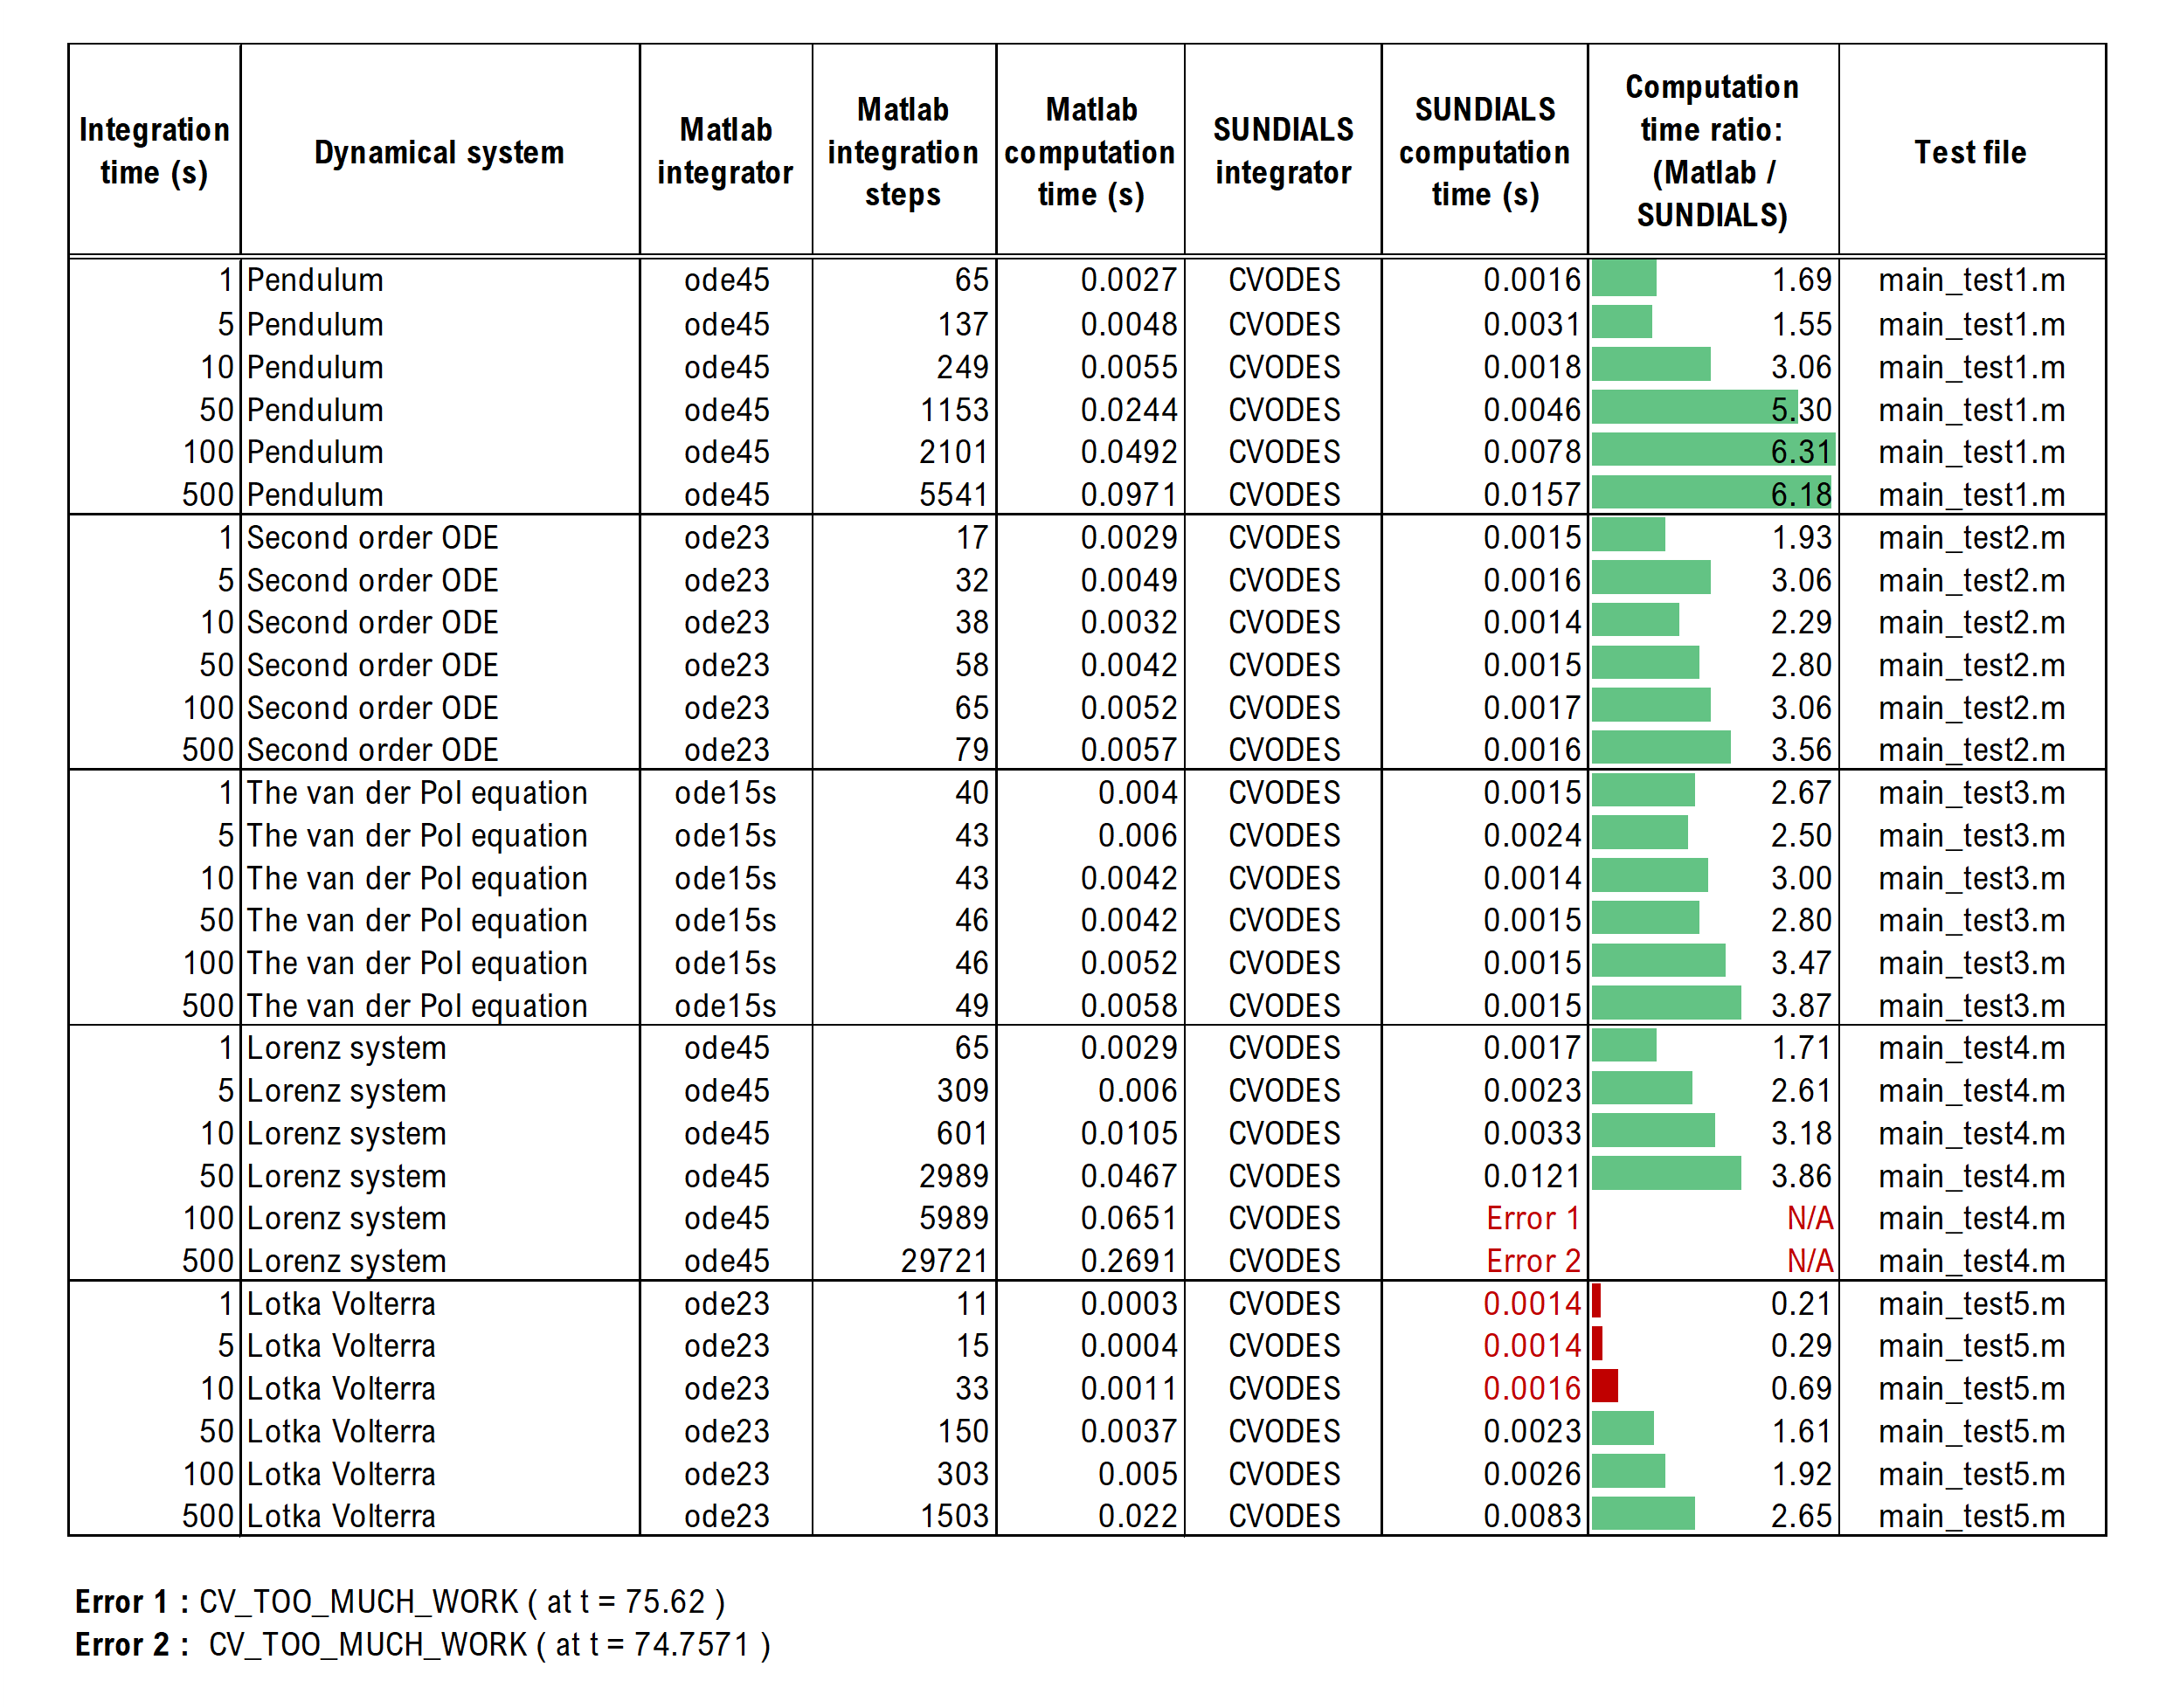
\includegraphics[scale=0.75]{images/table.png}
    \label{label_table}
\end{figure}

\begin{figure}[h!]
    \centering
    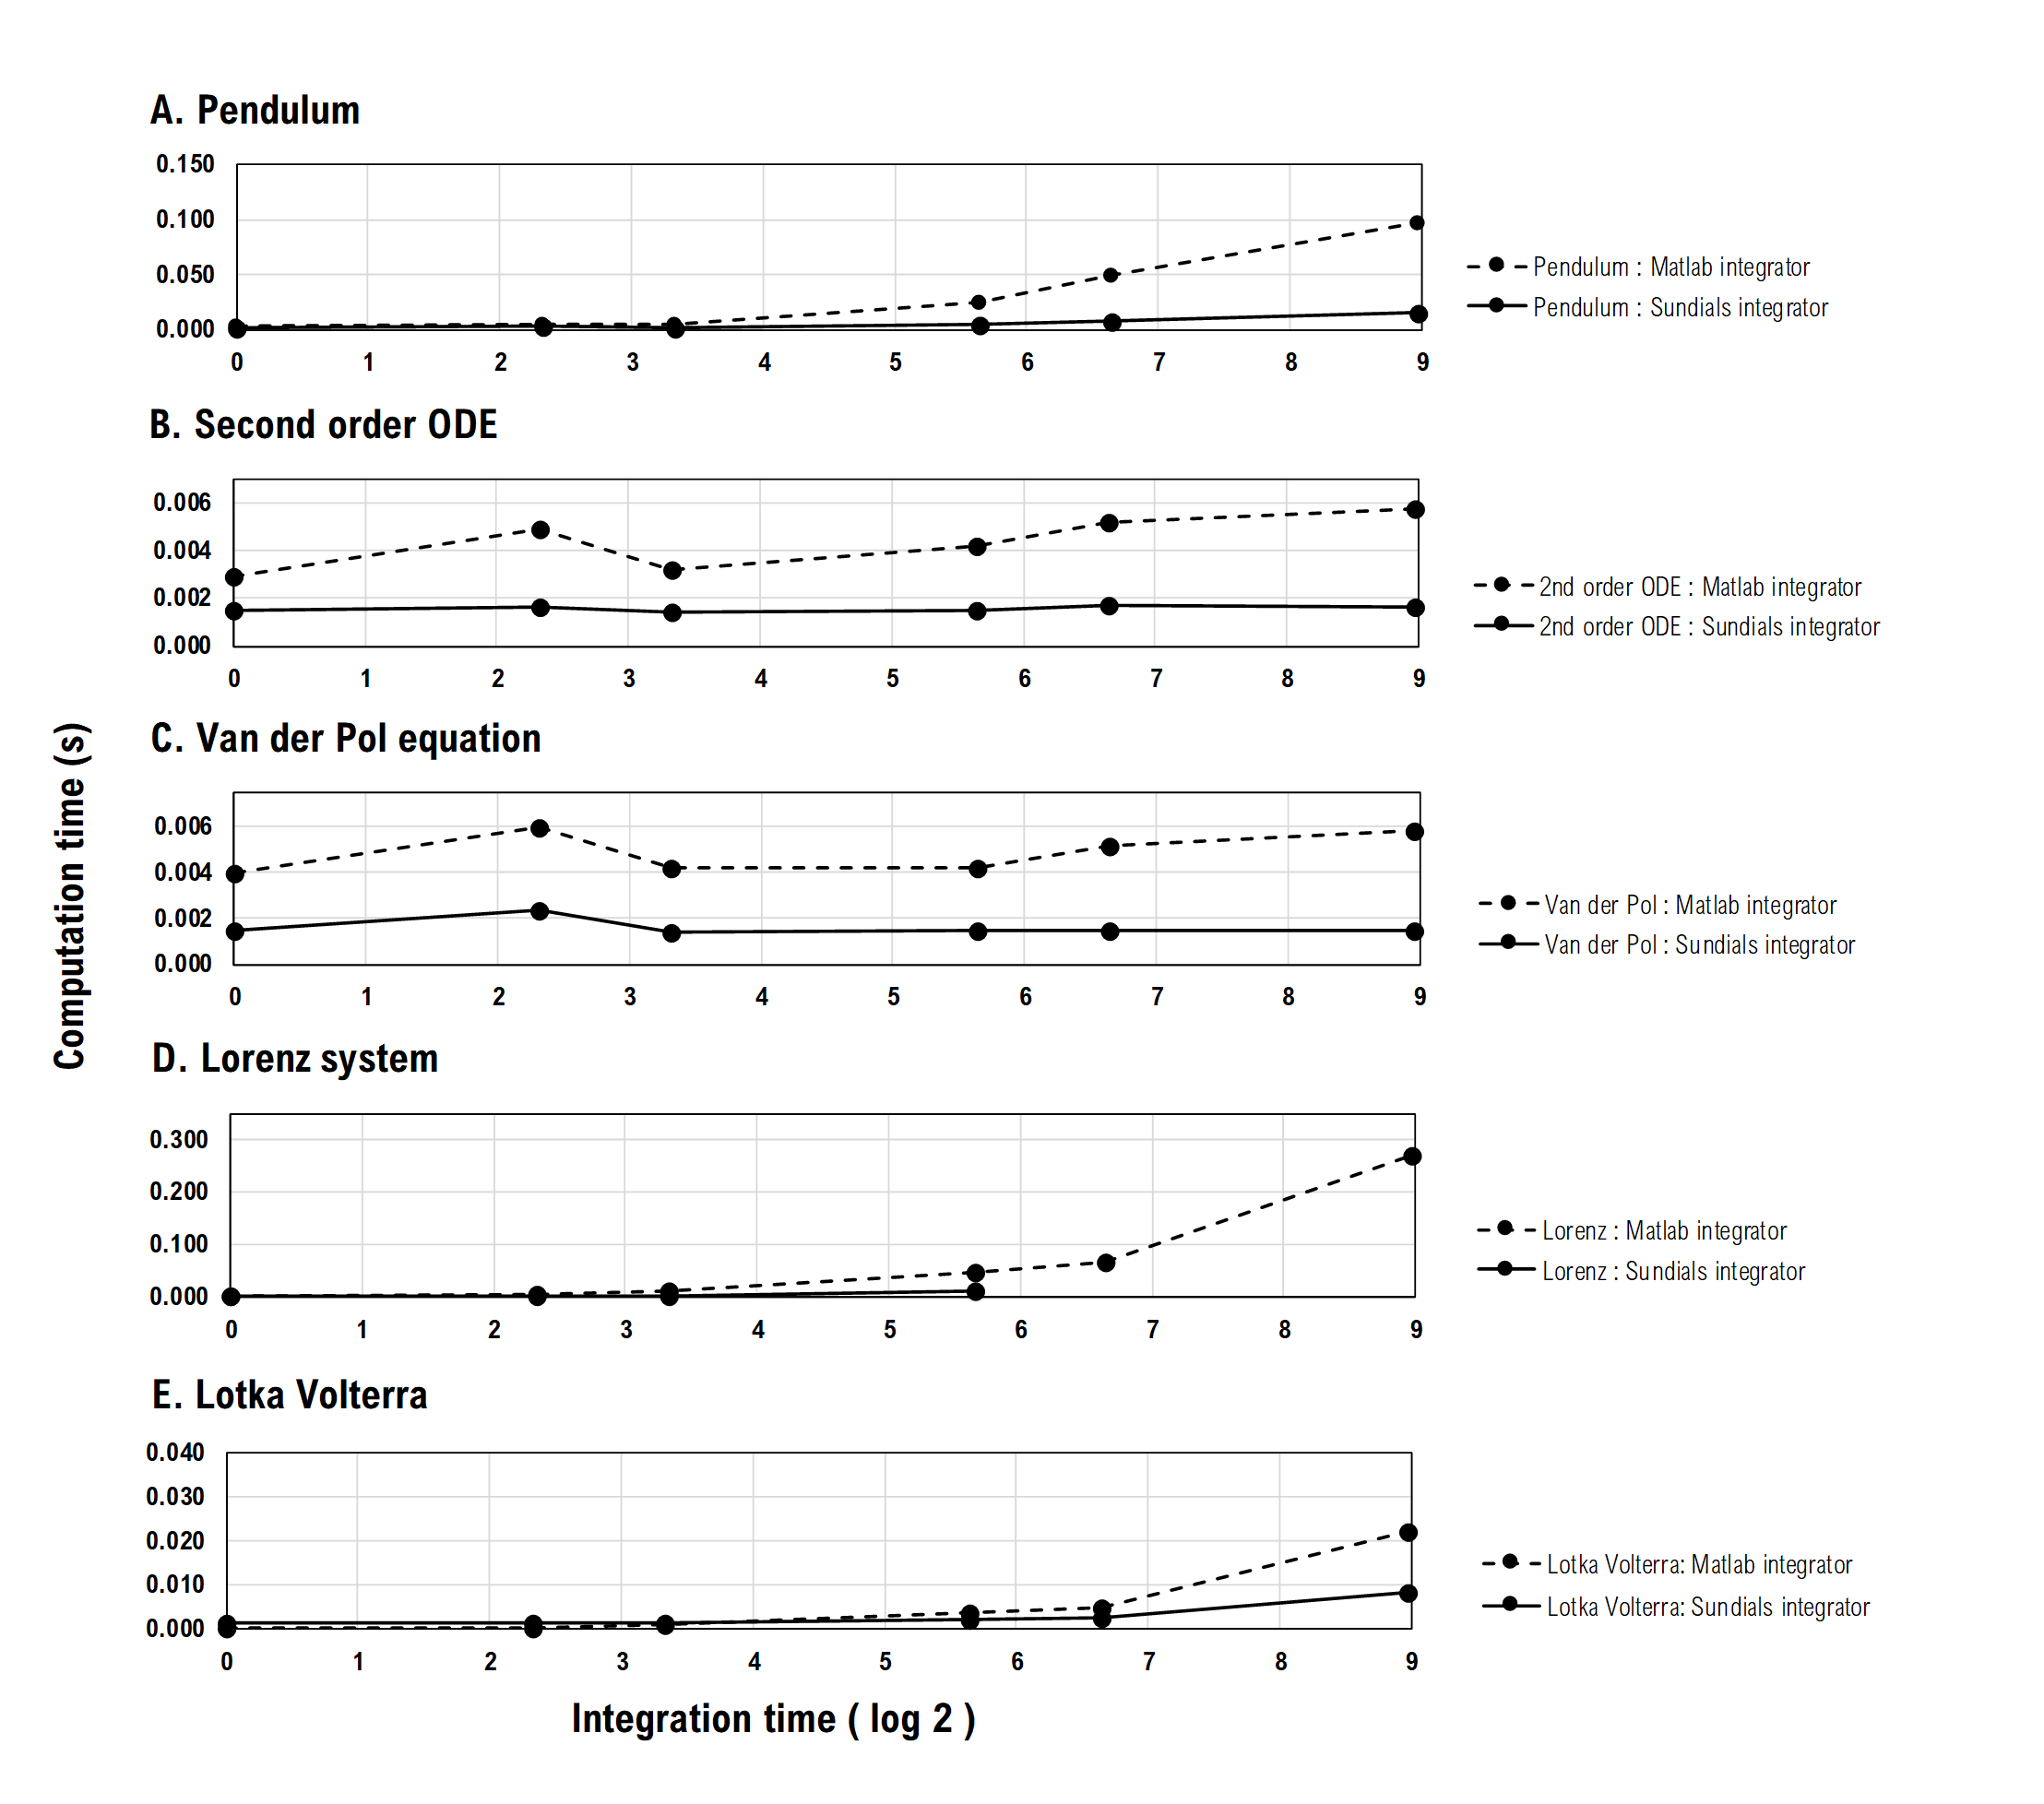
\includegraphics[scale=0.8]{images/chart.png}
    \label{label_chart}
\end{figure}


\section{Conclusions and Recommendations}
\label{conclusions_recommandations}

Explanation for example in \texttt{howToComputeMultipleJacobiansAtOnce.m}.

The following function is an object, which represents the mathematical
\begin{align}
  x(x_0,q).
\end{align}
It maps $\mathbb{R}^2 \times \mathbb{R}^2 \mapsto \mathbb{R}^2$.
\begin{lstlisting}[basicstyle=\small]
  I = casadi.integrator('I','cvodes',ode_struct,opts);
\end{lstlisting}

The object 
\begin{lstlisting}[basicstyle=\small]
  I_fwd = I.factory('I_fwd',{'x0','p','fwd:x0','fwd:p'},{'fwd:xf'}) 
\end{lstlisting}
represents the mathematical function
\begin{align}
  f(x_0,q_0, d_{x_0},d_{q}) = G_x(x_0,q) d_{x_0} + G_p (x_0,q) d_q.
\end{align}
It maps $\mathbb{R}^2 \times \mathbb{R}^2 \times \mathbb{R}^2 \times \mathbb{R}^2\mapsto \mathbb{R}^2$.
If we want to compute the full Jacobian, we need to evaluate the function four times. 
For every direction once. 
Casadi allows to do this by one function call with
\begin{align}
  f(x_0,q_0, \begin{bmatrix} 1 0 0 0  \\ 0 1 0 0 \end{bmatrix},\begin{bmatrix}  0 0 1 0  \\  0 0 0 1 \end{bmatrix}).
\end{align}
This is equivalent to 
\begin{align}
  f(
    \begin{bmatrix}
    x_0  x_0  x_0  x_0
    \end{bmatrix},
    \begin{bmatrix}
    q_0   q_0 q_0 q_0
    \end{bmatrix},
  \begin{bmatrix} 1 0 0 0  \\ 0 1 0 0 \end{bmatrix}
  ,\begin{bmatrix}  0 0 1 0  \\  0 0 0 1 \end{bmatrix}).
\end{align}
because internally $x_0$ and $q_0$ gets duplicated and the function $f$ is evaluated column wise.
In order to compute the Jacobian for multiple values, we need to duplicate the initial values and the directions as well.
To evaluate the Jacobian for $x_0^1,x_0^2x_0^3$ and $q_0^1, q_0^2, q_0^3$ we have to do the function call 
\begin{align}
  f(
    &\begin{bmatrix}
    x_0^1  x_0^1  x_0^1  x_0^1
    x_0^2  x_0^2  x_0^2  x_0^2
    x_0^3  x_0^3  x_0^3  x_0^3
    \end{bmatrix},  \\
    &\begin{bmatrix}
    q_0^1   q_0^1 q_0^1 q_0^1
    q_0^2   q_0^2 q_0^2 q_0^2
    q_0^3   q_0^3 q_0^3 q_0^3
    \end{bmatrix}, \\
    &\begin{bmatrix} 1 0 0 0  1 0 0 0 1 0 0 0 \\ 0 1 0 0 0 1 0 0 0 1 0 0\end{bmatrix}, \\
    &\begin{bmatrix}  0 0 1 0  0 0 1 0 0 0 1 0  \\   0 0 0 1  0 0 0 1 0 0 0 1 \end{bmatrix}).
\end{align}
and split up the result in the individual Jacobians afterwards.




\bibliography{References}
\bibliographystyle{plain}













\end{document}
